% Created 2018-06-21 Thu 12:30
\documentclass[8pt]{beamer}
% \usetheme{Montpellier}
% \usecolortheme{dove}

\usepackage[sc,osf]{mathpazo}   % With old-style figures and real smallcaps.
\linespread{1.025}              % Palatino leads a little more leading
% Euler for math and numbers
\usepackage[euler-digits,small]{eulervm}
%\documentclass[10pt]{llncs}
%\usepackage{llncsdoc}
\usepackage{minted}
\usepackage[utf8]{inputenc}
\usepackage[T1]{fontenc}
\usepackage{fixltx2e}
\usepackage{graphicx}
\usepackage{longtable}
\usepackage{float}
\usepackage{wrapfig}
\usepackage{rotating}
\usepackage[normalem]{ulem}
\usepackage{amsmath}
\usepackage{textcomp}
\usepackage{marvosym}
\usepackage{wasysym}
\usepackage{amssymb}
\usepackage{hyperref}
\usepackage{polynom}
\renewcommand{\mod}[1]{\left( \texttt{mod}~#1 \right)}
\newcommand{\N}{\mathbb N}
\newcommand{\Z}{\mathbb Z}
\newcommand{\Q}{\mathbb Q}
\newcommand{\C}{\mathbb C}
 % 'newunicodechar' for declaring things like alpha, beta, etc.
\usepackage[verbose]{newunicodechar}
\newunicodechar{λ}{\ensuremath{\lambda}}

\newcommand{\degree}{\texttt{degree}}
\tolerance=1000
% \usetheme{Antibes}
\author{Siddharth Bhat}
\date{July 31st, 2023}
\institute{MSR \\ AI4Code}
\title{Learning Program Synthesis for Integer Sequences}
% \hypersetup{
%   pdfkeywords={},
%   pdfsubject={},
%   pdfcreator={Emacs 24.5.1 (Org mode 8.2.10)}}
\expandafter\def\expandafter\insertshorttitle\expandafter{%
  \insertshorttitle\hfill%
  \insertframenumber\,/\,\inserttotalframenumber}

\begin{document}


\maketitle

\begin{frame}[fragile]{The Problem}
\begin{itemize}
\item Given an OEIS sequence $s$, generate a program $p$ such that $s_i = p(i)$. \pause
\end{itemize}
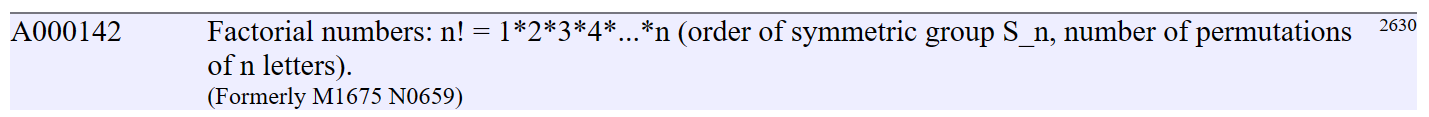
\includegraphics[width=\textwidth]{./catalan-1.png} \pause
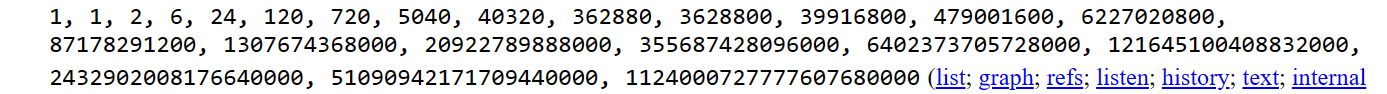
\includegraphics[width=\textwidth]{./catalan-2.png} \pause
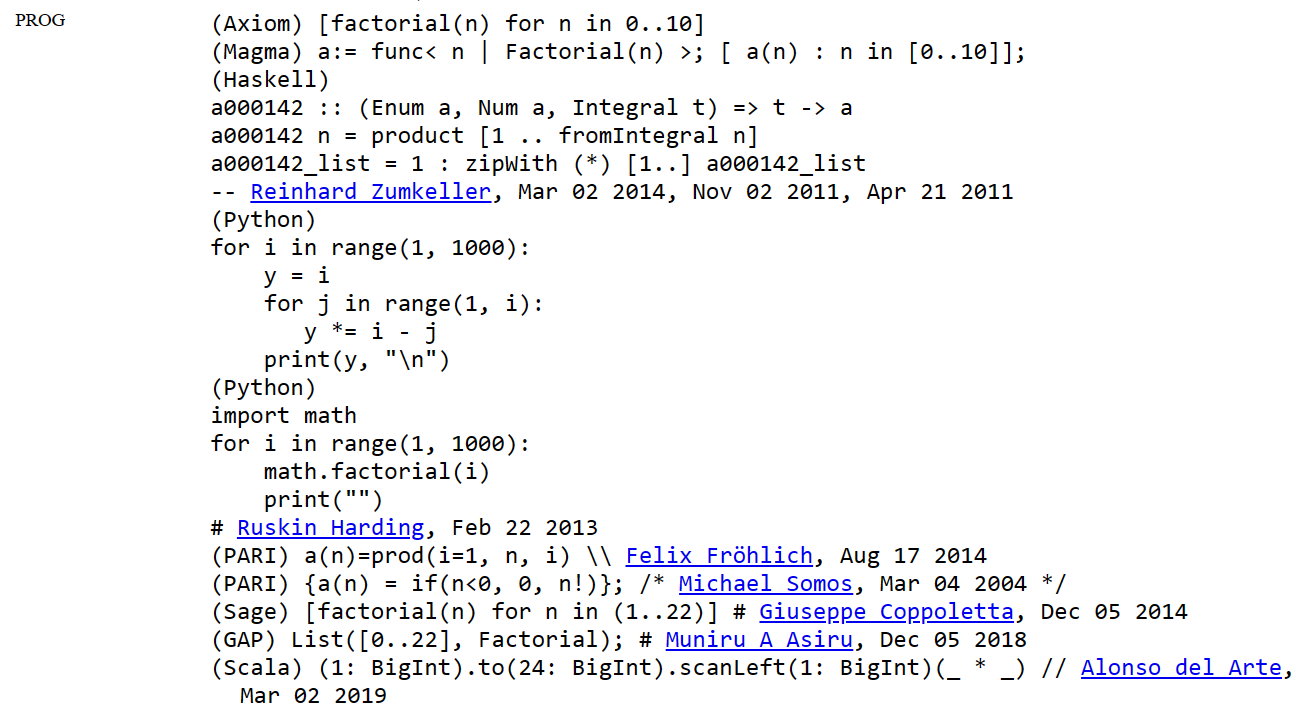
\includegraphics[width=\textwidth]{./catalan-3.png} \pause
\end{frame}

\begin{frame}[fragile]{The Problem Statement}
\begin{itemize}
\item Given an OEIS sequence $s$, generate a program $p$ such that $s_i = p(i)$. \pause
\item What language is $p$ written in? 
\item What is our training data set of $(s, p)$ pairs?
\item What is our architecture for generating a program $p_t$ for a novel sequence $t$ during test time?
\end{itemize}
\end{frame}


\begin{frame}[fragile]{Programming Language}
\begin{minted}{python}
P := 0 | 1 | x | y | P + P | P - P | P * P | P div P | P mod P
\end{minted}
\pause
\begin{minted}{python}
   |  cond(P, P, P) # cond(c, t, e) := return t if c else e
\end{minted}
\pause
\begin{minted}{python}
F := lambda (x, y). P
\end{minted}
\pause
\begin{minted}{python}
P := 
| loop(f, a, b)
# loop(F, P, P) := 
#   while a > 0: 
#     b = f(a, b)
#     a -= 1
#   return b;
\end{minted}
\pause
\begin{itemize}
\item For OEIS example, let sequence be $s_n \equiv n!$. \pause
\item This is given by the recurrence $s_0 = 1$, $s_{n+1} = n \cdot s_n$ \pause
\item This is the program \texttt{loop(λ(x,y).x*y, x, 1)}. \pause
\item This is the program \texttt{loop(λ(counter,accum). counter*accum, counter=n, start=1)}. \pause
\end{itemize}
\end{frame}


\begin{frame}{Dataset Generation: A Program for an OEIS sequence $s$}
\begin{itemize}
\item Idea: generate a program in reverse polish notation! \pause
\item $1 + (2 * 3) \mapsto \texttt{"1 2 3 * +"}$ \pause 
\item $[] \pause \mapsto_1 [1] \pause \mapsto_2 [1;2] \pause \mapsto_3 [1;2;3] \pause \mapsto_* [1; (2*3)] \pause \mapsto_+ [1+(2*3)]$ \pause
\item $(1 + 2) * 3 \mapsto \texttt{"1 2 + 3 *"}$ \pause
\item $[] \pause \mapsto_1 [1] \pause \mapsto_2 [1;2] \pause \mapsto_+ [(1+2)] \pause \mapsto_3 [(1+2);3] \pause \mapsto_* [(1+2)*3]$ 
\item For OEIS example, let sequence be $s_n \equiv n!$. \pause
\item This is given by the recurrence $s_0 = 1$, $s_{n+1} = n \cdot s_n$ \pause
\item This is the program \texttt{loop(λ(x,y).x*y, x, 1)}. \pause
\item A valid program generation is $[] \pause \mapsto_x [x] \pause \mapsto_y [x;y] \pause \mapsto_{*} [x*y] \pause \mapsto_x [x*y;x] \pause \mapsto_{1} [x*y;x;1] \mapsto_{loop} [loop(λ(x,y).x*y, x, 1)]$ \pause
\item Generate program, test if program matches sequence for some finite sequence length (say, 100).
  Check that $s_i =_? p(i)$ for $0 \leq i \leq 100$. \pause
\item Randomly explore space of possible programs.
\end{itemize}
\end{frame}

\begin{frame}{Training from the Dataset}
\begin{itemize}
\item Consider the sequence $s_i \equiv i!$. ($s \equiv [1, 2, 6, 24, \dots]$). \pause
\item We found the action sequence $[] \mapsto_x [x] \pause \mapsto_y [x;y] \pause \mapsto_{*} [x*y] \mapsto_x [x*y;x] \mapsto_{1} [x*y;x;1] \mapsto_{loop} [loop(λ(x,y).x*y, x, 1)]$. \pause
\item This is the program $p \equiv \texttt{loop(λ(x,y).x*y, x, 1)}$ such that $s_i = p(i)$.\pause
\item We want to learn the function:
\begin{tabular}{rll}
Program Stack & Sequence & Next Action \\
$[]$ & $[1, 2, 6, 24, \dots]$ & $\mapsto_x$ \pause \\
$[x]$ & $[1, 2, 6, 24, \dots]$ & $\mapsto_y$ \pause \\
$[x;y]$ & $[1, 2, 6, 24, \dots]$ & $\mapsto_*$ \\
$[x*y;x]$ & $[1, 2, 6, 24, \dots]$ & $\mapsto_1$ \\
$[x*y;x;1]$ & $[1, 2, 6, 24, \dots]$ & $\mapsto_{loop}$ \\
$[loop(λ(x,y).x*y, x, 1)]$ & $[1, 2, 6, \dots]$ & $\mapsto_{\blacksquare}$ \\
\end{tabular}

\item Learn this function using an NN. \pause
\item \textbf{Input}: embedding of current program stack + embedding of first 16 terms of OEIS sequence. \pause
\item \textbf{Output:} one-hot vector over next actions.
\end{itemize}
\end{frame}


\begin{frame}[fragile]{Embeddings in Greater Detail}
% \includegrapics{./embedding.png} \pause
\begin{itemize}
\item $\texttt{[x*y;x]} \quad \texttt{[1, 2, 6, 24]} \mapsto_1 ? $ \pause 
\end{itemize}
\begin{tabular}{ll}
Embedding Computation & Data Embedded  \\
\texttt{action\_onehot = NNPolicy(vprogram, vseq)} & $\texttt{[x*y;x]} \quad \texttt{[1, 2, 6, 24]} \mapsto_1 ? $ \pause  \\
\texttt{v1 = NNProgramMul(NNVarEmbed(x), NNVarEmbed(y))} & \texttt{x*y} \pause \\
\texttt{vprogram = NNProgramCons(v1, VarEmbed(x))} & \texttt{[(x*y); x]} \pause \\
\texttt{v3 = NNSequenceCons(NNNumber(6), NNNumber(24))} & \texttt{[6; 24]} \pause \\
\texttt{v4 = NNSequenceCons(NNNumber(2), v3)}  & \texttt{[2; 6; 24]} \pause \\
\texttt{vseq = NNSequenceCons(NNNumber(1), v4)}  & \texttt{[1; 2; 6; 24]} \pause \\
\end{tabular}
\end{frame}


\begin{frame}{Evaluation}
\begin{itemize}
\item How many OEIS sequences from the set of all sequences $S$ have valid programs generated for them? (timeout=10min) \pause
\item Pick an OEIS sequence $s \in S$. Try to generate program $p$ such that $p(i) = s_i$ for 10 minutes. Fail if sequence was not generated. \pause
\item Generation $0$: Random exploration of program space. Generates 993 solutions. \pause
\item Use Generation $0$ to learn policy. Run generation $1$. \pause
\item Generation 1 discovers additional 8483 solutions. \pause
\item Use generation $k$ to learn policy. Run generation $k+1$. \pause
\end{itemize}
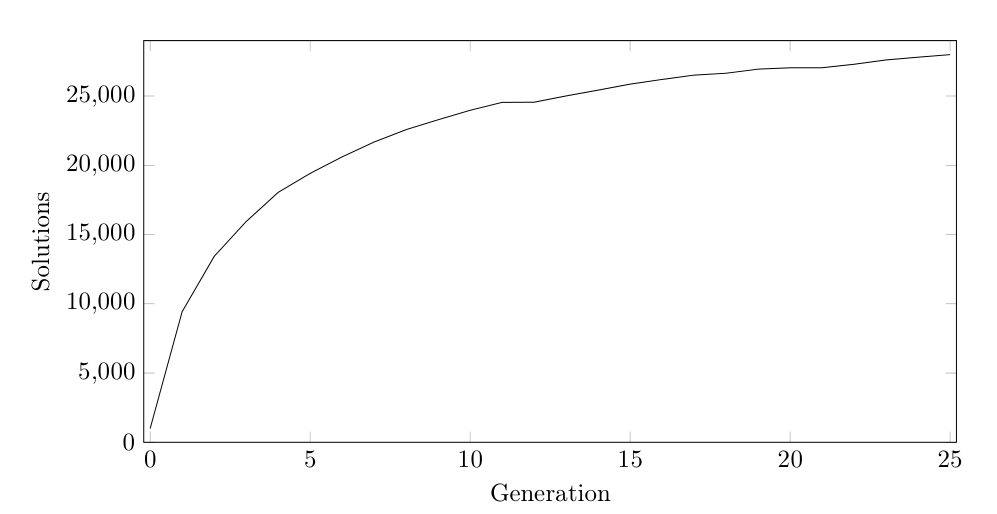
\includegraphics[width=\textwidth]{./plot-1.png} \pause
\end{frame}

\begin{frame}[fragile]{Occam's Razor}
\begin{itemize}
\item When building dataset, if two programs $p_1, p_2$ are found for sequence $s$, keep the smaller one. \pause
\item Baseline dataset: always pick smallest program that generates a sequence $s$. \pause
\item Ablated dataset: pick random program that generates a sequence $s$.  \pause
\item Model trained on ablated dataset generates 10\% fewer programs! \pause
\end{itemize}
\begin{quote}
Thus, we can say that selecting the smallest solutions instead of the random ones for training
helps finding new solutions in later generations. 
\end{quote}
\end{frame}

\begin{frame}[fragile]{\texttt{Conclusion}}
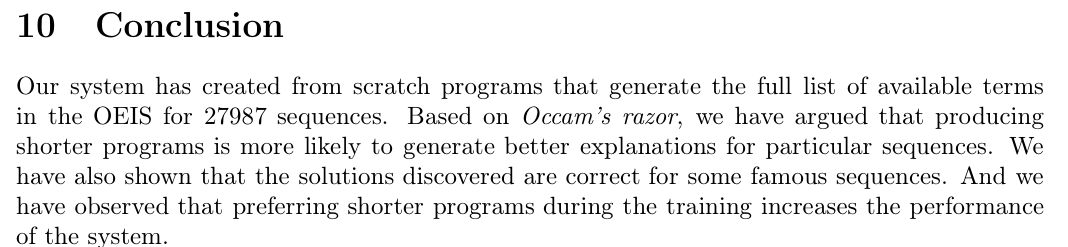
\includegraphics{conclusion.png}
\end{frame}

\begin{frame}[fragile]{Fancier Dataset Construction}
\begin{itemize}
\item No need to pick a sequence $s$ and then try to randomly generate programs for it. \pause
\item Can start by randomly generating programs with tree search, and then matching these programs to known sequences. \pause
\item Also provides automatic caching: If we try to produce a node that already exists, skip the node. \pause
\end{itemize}
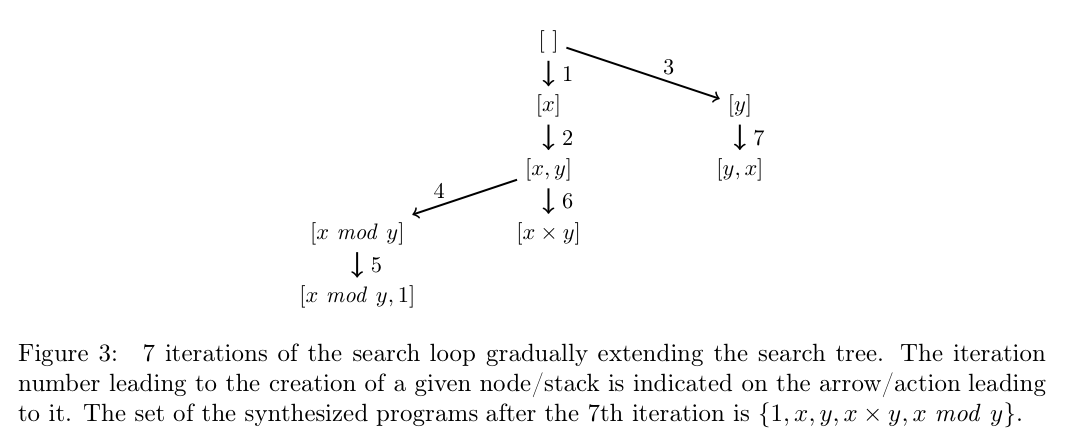
\includegraphics[width=\textwidth]{./tree-1.png} \pause
\end{frame}


\begin{frame}[fragile]{\texttt{compr}}
\begin{minted}{python}
compr(f, a) := 
| failure if a < 0 
| min{ m | m >= 0 and f(m, 0) <= 0 } if a = 0
| min{ m | m > compr(f, a-1) and f(m, 0) <= 0} otherwise
\end{minted}
\end{frame}

\end{document}
# (f: ZxZ -> Z) x (a : Z) -> Z
